\documentclass[12pt]{article}
\usepackage[utf8]{inputenc}

\title{ARM-Thumb Machine Code Reference}
\author{Michael Lyle}
\date{October 2021}

\ttfamily

\usepackage[
  letterpaper,
  twoside,
  bindingoffset=0.7cm,
  inner=1.8cm,
  outer=1.8cm,
  top=2cm,
  bottom=2cm,
  headsep=1.2cm
]{geometry}

\usepackage[final]{pdfpages}
\usepackage{graphicx}
\usepackage{imakeidx}
\makeindex

\newcommand{\fullrule}{\\[-4pt]\noindent\rule{\textwidth}{1pt}\\}

\newcommand{\instruction}[5]{\addcontentsline{toc}{subsection}{#1}\vspace{0.8cm}\noindent \textbf{#1}\index{#5}\hspace*{\fill}\texttt{#3}\fullrule#2\vspace{0.25cm}\begin{center}#4\end{center}}

\newcommand{\hexnum}[2]{$\mathtt{#1}_{16}$ ($\mathtt{#2}_{10}$)}
\newcommand{\numtt}[1]{$\mathtt{#1}$}
\newcommand{\reg}[1]{$r#1$}


\setlength{\parindent}{0pt}

\begin{document}

\maketitle
\tableofcontents
\vspace{5.5cm}
\begin{center}
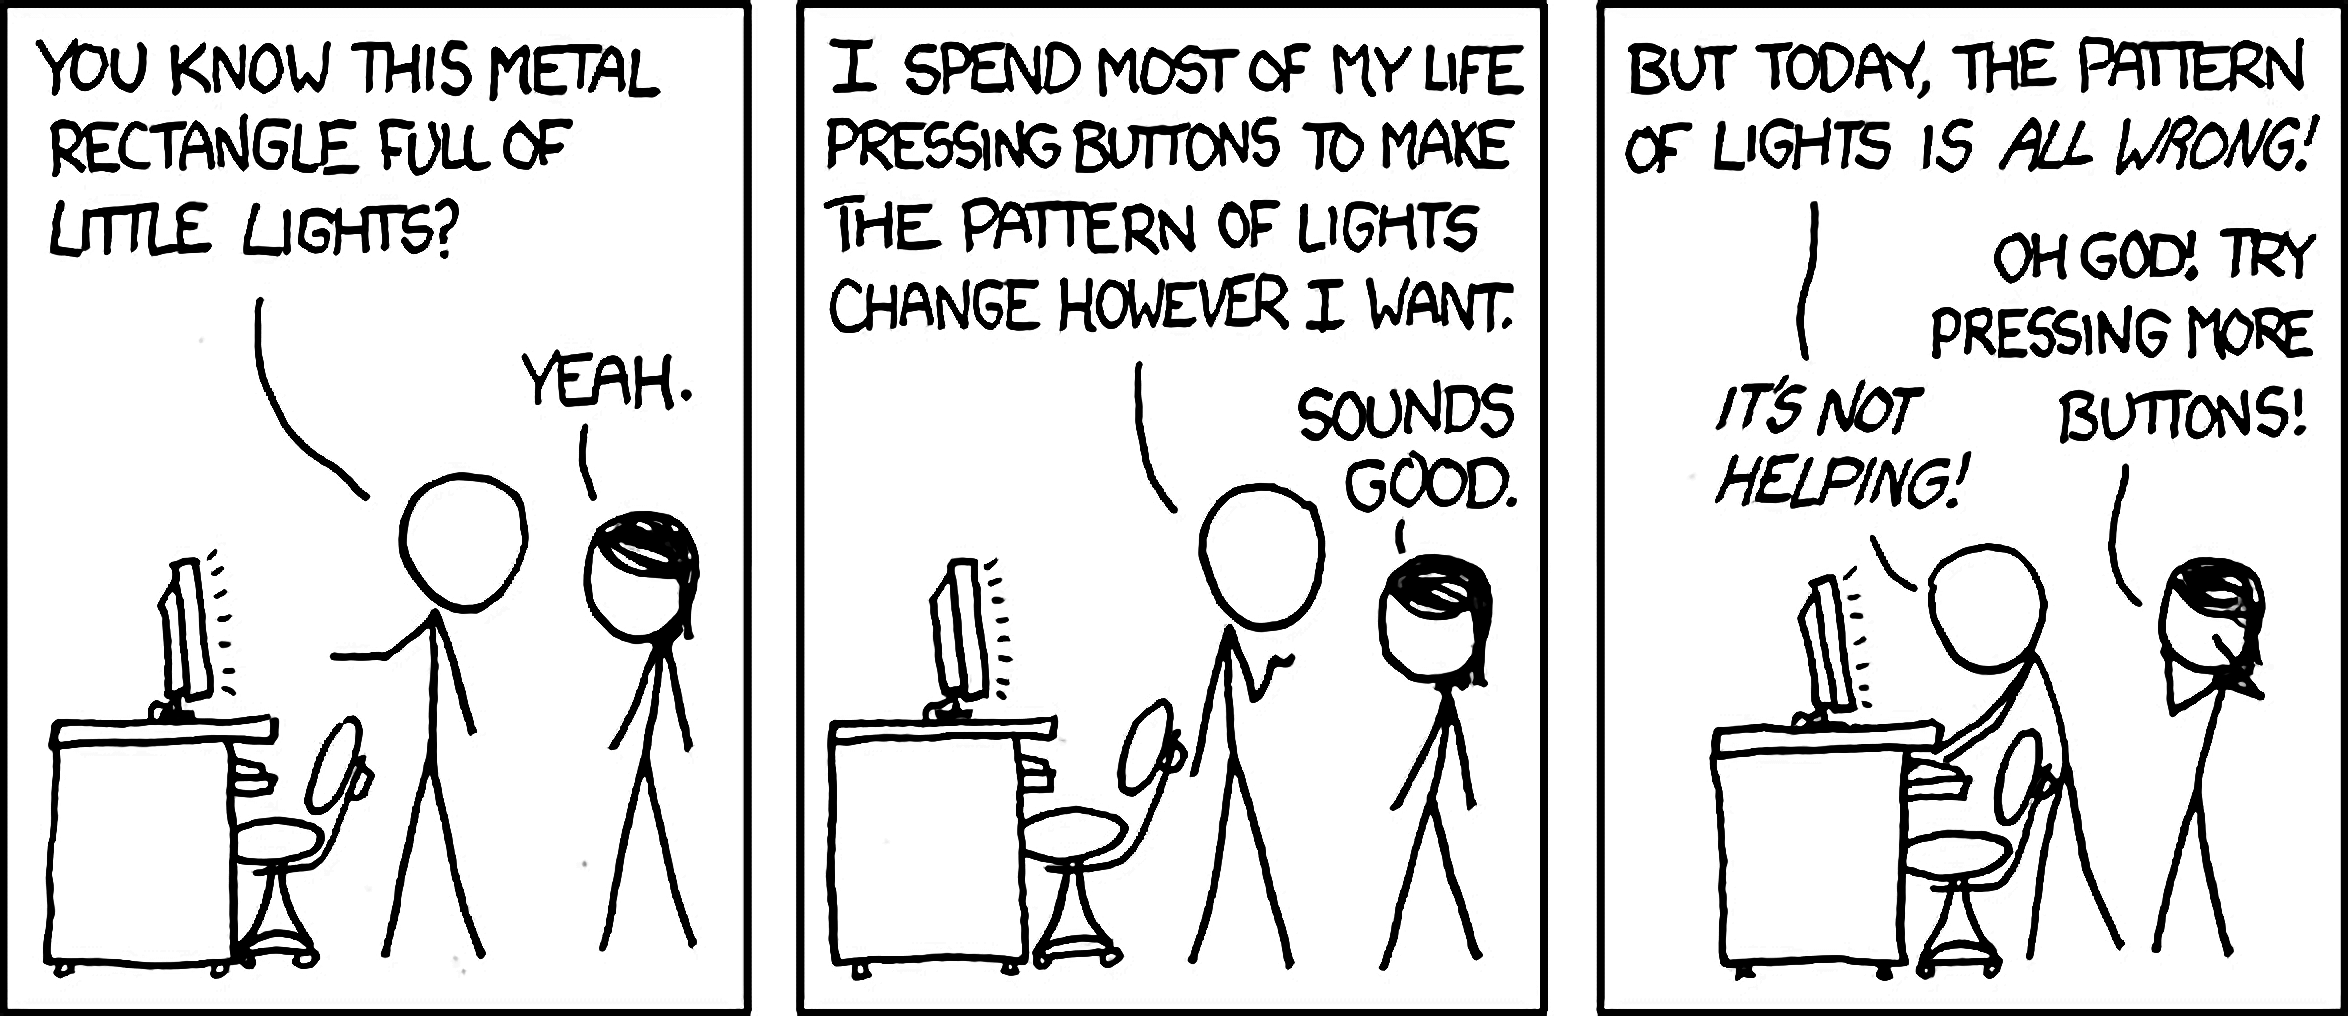
\includegraphics[width=5.25in]{computer_problems.png}

\scriptsize{XKCD \#722, "Computer Problems" (by Randall Munroe)}
\end{center}

\newpage

\section{Architecture Summary}

In this course, we will be learning ARM Thumb machine language.  ARM is one of the most common instruction set architectures in the world.\vspace{0.5cm}

It is used in almost all cellular phones, most tablets, and many laptop computers, in addition to a large share of the microcontrollers in cars and everyday items. \vspace{0.5cm}

ARM Thumb is a portion of the instruction set consisting of $16$ bit long instructions.  Normal ARM instructions are $32$ bits long, but we will not use them in this class.\vspace{0.5cm}

Specifically, we are writing code for the ARMv7 Thumb architecture.  Its characteristics are:

\begin{itemize}
    \item 32-bit (4 byte) register (word) size
    \item 32-bit (4 byte) address size
    \item 16-bit (2 byte) instruction length
    \item \index{address}Addresses point to individual bytes.  Instructions and words should be aligned in memory.
    \begin{itemize}
        \item An address pointing aligned with the beginning of a word will end in $0$, $4$, $8$, or $C$ in base $16$.
        \item An address pointing to an instruction will end in $0$, $2$, $4$, $6$, $8$, $A$, $C$, or $E$ in base $16$.
    \end{itemize}
    \item Instructions can access memory, or perform arithmetic, but not both (RISC / load-store machine).
    \item Eight general-purpose registers are easily accessed (\reg{0}-\reg{7}).
    \item Five additional general-purpose registers are more difficult to access (\reg{8}-\reg{12})
    \item Three special purpose registers (stack pointer, link register, and program counter)
    \item Capable ALU with hardware multiplier and standard flags:
    \begin{itemize}
        \item N (negative),
        \item Z (zero),
        \item C (carry),
        \item and V (overflow)
    \end{itemize}
\end{itemize}

\subsection{Machine Language vs. Assembly Language}

In this course, we are writing programs in machine language.  This is a raw sequence of numbers that tells the computer what to do.
\vspace{0.5cm}

One step up from machine language is to use assembly language, where we write one line of code for each instruction, and the assembler translates this into machine language.  Assemblers make this process slightly easier by handling the details of instruction encoding and calculating addresses for the programmer.

\newpage

\section{ARM-Thumb Basic Instructions}

The following are just a few of the many instructions in the ARM-Thumb instruction set.  There are enough instructions in this manual to be able to write any program.  In other words, this set of instructions are Turing-complete.  But other instructions, not listed here, are often necessary to write the shortest and fastest possible program.

\instruction{ADD (add immediate)}{Add an 8 bit value (included in the instruction) to a register.  Flags are updated based on the result value.}{0011 0ddd iiii iiii}{$r[d] = r[d] + i$}{add}
\index{immediate instructions}
\begin{tabular}{p{0.15\textwidth} p{0.10\textwidth} p{0.63\textwidth}}
\texttt{ddd} & (3 bits) & This is the register number of the operand to add to, \underline{and} the destination register where the result should be placed. \\
\texttt{iiii iiii} & (8 bits) & This is the value that should be added, included as an immediate operand in the instruction. \\
\end {tabular}

\vspace{1cm}


Examples:

\begin{tabular}{p{0.33\textwidth} p{0.09\textwidth} p{0.44\textwidth}}
\texttt{0011 0ddd iiii iiii}&3???&Basic instruction encoding\\
\hline
\texttt{0011 0000 0000 0001}&3001&Adds the number \numtt{1} to \reg{0} \\
\hline
\texttt{0011 0011 0001 0010}&3312&Adds the number \hexnum{12}{18} to \reg{3} \\
\hline
\texttt{0011 0111 1010 0101}&37A5&Adds the number \hexnum{A5}{165} to \reg{7} \\
\hline

\end{tabular}


\instruction{ADD (add registers)}{Add two registers together, storing the result in a (optionally different) third register.  Flags are updated.}{0001 100m mmnn nddd}{$r[d] = r[m] + r[n]$}{add}

\begin{tabular}{p{0.15\textwidth} p{0.10\textwidth} p{0.63\textwidth}}
\texttt{mmm} & (3 bits) & This is the register number of the first operand to add. \\
\texttt{nnn} & (3 bits) & This is the register number of the second operand to add. \\
\texttt{ddd} & (3 bits) & This is the register number to store the result in. \\
\end {tabular}

\vspace{1cm}


Examples:

\begin{tabular}{p{0.33\textwidth} p{0.09\textwidth} p{0.44\textwidth}}
\texttt{0001 100m mmnn nddd}&1???&Basic instruction encoding\\
\hline
\texttt{0001 1000 0000 0000}&1800&Adds \reg{0} to register \reg{0} and stores the result in \reg{0} (doubles \reg{0})\\
\hline
\texttt{0001 1000 0101 0011}&1853&Adds \reg{1} to \reg{2} and stores the result in \reg{3} \\
\hline
\texttt{0001 1000 1000 1011}&188B&Adds \reg{2} to \reg{1} and stores the result in \reg{3} (same as above)\\
\hline
\end{tabular}

\newpage
\instruction{B (branch)}{Branches the program counter to a new location.  (Goto a different part of your program)}{1110 0iii iiii iiii}{$pc = pc + 2*(i+2)$}{branch}

\begin{tabular}{p{0.15\textwidth} p{0.10\textwidth} p{0.63\textwidth}}
\texttt{iiiiiiii...} & (11 bits) & Number of instructions to jump forward (or backwards, if negative...)\\
\end {tabular}

\vspace{1cm}


Examples:

\begin{tabular}{p{0.33\textwidth} p{0.09\textwidth} p{0.44\textwidth}}
\texttt{1110 0iii iiii iiii}&E???&Basic instruction encoding\\
\hline
\texttt{1110 0111 1111 0000}&E7F0&Goes back to 14 instructions before this one.\\
\hline
\texttt{1110 0111 1111 0001}&E7F1&Goes back to 13 instructions before this one.\\
\hline
\texttt{1110 0111 1111 0010}&E7F2&Goes back to 12 instructions before this one.\\
\hline
\texttt{1110 0111 1111 1100}&E7FC&Goes back to 2 instructions before this one.\\
\hline
\texttt{1110 0111 1111 1101}&E7FD&Goes back to 1 instructions before this one.\\
\hline
\texttt{1110 0111 1111 1110}&E7FE&Goes to \textbf{THIS} instruction (infinite loop)\\
\hline
\texttt{1110 0111 1111 1111}&E7FF&Goes to the instruction after this one (does nothing)\\
\hline
\texttt{1110 0000 0000 0000}&E000&Skips 1 instruction after this one\\
\hline
\texttt{1110 0000 0000 0001}&E001&Skips 2 instructions after this one\\
\hline
\texttt{1110 0000 0000 0010}&E002&Skips 3 instructions after this one\\
\hline
\texttt{1110 0000 0000 1111}&E00F&Skips 16 instructions after this one\\
\hline
\end{tabular}

\instruction{CMP (compare registers)}{Subtracts one register from another and updates flags.  The result of the subtraction is thrown away. }{0100 0010 10mm mnnn}{$tmp = r[n] - r[m]$}{compare}

\begin{tabular}{p{0.15\textwidth} p{0.10\textwidth} p{0.63\textwidth}}
\texttt{nnn} & (3 bits) & This is the register number of the operand to subtract from. \\
\texttt{mmm} & (3 bits) & This is the register number of the subtrahend \\
\end{tabular}
\vspace{1cm}

Examples:

\begin{tabular}{p{0.33\textwidth} p{0.09\textwidth} p{0.44\textwidth}}
\texttt{0100 0010 10mm mnnn}&42??&Basic instruction encoding\\
\hline
\texttt{0100 0010 1000 0001}&4281&Subtracts \reg{0} from register \reg{1} and updates flags \\
\hline
\texttt{0100 0010 1011 1110}&42BE&Subtracts \reg{7} from register \reg{6} and updates flags \\
\hline
\end{tabular}

\newpage
\instruction{MOV (move immediate)}{Moves a value, provided in the instruction, into a chosen register.}{0010 0ddd iiii iiii}{$r[d] = i$}{move}
\index{immediate instructions}

\begin{tabular}{p{0.15\textwidth} p{0.10\textwidth} p{0.63\textwidth}}
\texttt{ddd} & (3 bits) & This is the register number where the result should be placed. \\
\texttt{iiii iiii} & (8 bits) & This is the value that should be placed into the destination register.  The high 24 bits of the register will be $0$ and the remaining 8 bits will be the immediate value. \\
\end {tabular}

\vspace{1cm}


Examples:

\begin{tabular}{p{0.33\textwidth} p{0.09\textwidth} p{0.44\textwidth}}
\texttt{0010 0ddd iiii iiii}&2???&Basic instruction encoding\\
\hline
\texttt{0010 0000 0000 0000}&2000&Sets \reg{0} to the value \numtt{0}\\
\hline
\texttt{0010 0111 1111 1111}&27FF&Sets \reg{7} to the value \hexnum{FF}{255} \\
\hline
\texttt{0010 0010 0000 0101}&2205&Puts the number \numtt{5} in \reg{2} \\
\hline

\end{tabular}

\instruction{MOV (move register)}{Copies a value from one register to another.}{0100 0110 00mm mddd}{$r[d] = r[m]$}{move}

\begin{tabular}{p{0.15\textwidth} p{0.10\textwidth} p{0.63\textwidth}}
\texttt{mmm} & (3 bits) & This is the register number from which the value should be copied. \\
\texttt{ddd} & (3 bits) & This is the register number where the value should be placed.
\end{tabular}
\vspace{1cm}

Examples:

\begin{tabular}{p{0.33\textwidth} p{0.09\textwidth} p{0.44\textwidth}}
\texttt{0100 0110 00mm mddd}&46??&Basic instruction encoding\\
\hline
\texttt{0100 0110 0000 1000}&4608&Sets \reg{0} to the value in \reg{1}\\
\hline
\texttt{0100 0110 0000 0001}&4601&Sets \reg{1} to the value in \reg{0}\\
\hline
\texttt{0100 0110 0011 1110}&463E&Sets \reg{6} to the value of \reg{7}\\
\hline
\end{tabular}

\newpage
\instruction{MUL (multiply registers)}{Multiplies register $n$ by register $d$, and stores the result in register $d$.}{0100 0011 01nn nddd}{$r[d] = r[d] * r[n]$}{multiply}

\begin{tabular}{p{0.15\textwidth} p{0.10\textwidth} p{0.63\textwidth}}
\texttt{nnn} & (3 bits) & This is the register number that contains the first number to be multiplied. \\
\texttt{ddd} & (3 bits) & This is the register number with the second multiplicand, and where the value should be placed.
\end{tabular}
\vspace{1cm}

Examples:


\begin{tabular}{p{0.33\textwidth} p{0.09\textwidth} p{0.44\textwidth}}
\texttt{0100 0011 01nn nddd}&43??&Basic instruction encoding\\
\hline
\texttt{0100 0011 0100 0000}&4340&Squares \reg{0} and puts the result back in \reg{0}\\
\hline
\texttt{0100 0011 0100 1000}&4348&Sets \reg{0} to \reg{1} times \reg{0}\\
\hline
\texttt{0100 0011 0100 0001}&4341&Sets \reg{1} to \reg{1} times \reg{0}\\
\hline
\texttt{0100 0011 0110 0011}&4363&Sets \reg{3} to \reg{3} times \reg{4}\\
\hline
\end{tabular}

\instruction{SUB (subtract immediate)}{Subtract an 8 bit value (included in the instruction) from a register.  Flags are updated based on the result value.}{0011 1ddd iiii iiii}{$r[d] = r[d] - i$}{subtract}
\index{immediate instructions}

\begin{tabular}{p{0.15\textwidth} p{0.10\textwidth} p{0.63\textwidth}}
\texttt{ddd} & (3 bits) & This is the register number of the operand to subtract from, \underline{and} the destination register where the result should be placed. \\
\texttt{iiii iiii} & (8 bits) & This is the value that should be subtracted, included as an immediate operand in the instruction. \\
\end {tabular}

\vspace{1cm}


Examples:

\begin{tabular}{p{0.33\textwidth} p{0.09\textwidth} p{0.44\textwidth}}
\texttt{0011 1ddd iiii iiii}&3???&Basic instruction encoding\\
\hline
\texttt{0011 1000 0000 0001}&3801&Subtracts the number \numtt{1} to \reg{0} \\
\hline
\texttt{0011 1011 0011 0001}&3B32&Subtracts the number \hexnum{32}{50} from \reg{3} \\
\hline
\texttt{0011 1111 1010 0101}&3FA5&Subtracts the number \hexnum{A5}{165} from \reg{7} \\
\hline

\end{tabular}

\newpage
\instruction{SUB (subtract registers)}{Subtract one register from another, storing the result in a (optionally different) third register.  Flags are updated.}{0001 101m mmnn nddd}{$r[d] = r[n] - r[m]$}{subtract}

\begin{tabular}{p{0.15\textwidth} p{0.10\textwidth} p{0.63\textwidth}}
\texttt{nnn} & (3 bits) & This is the register number of the operand to subtract. \\
\texttt{nnn} & (3 bits) & This is the register number of the operand to subtract from. \\
\texttt{ddd} & (3 bits) & This is the register number to store the result in. \\
\end {tabular}

\vspace{1cm}


Examples:

\begin{tabular}{p{0.33\textwidth} p{0.09\textwidth} p{0.44\textwidth}}
\texttt{0001 101m mmnn nddd}&1???&Basic instruction encoding\\
\hline
\texttt{0001 1010 0000 0000}&1A00&Subtracts \reg{0} from register \reg{0} and stores the result in \reg{0} (sets \reg{0} to \numtt{0})\\
\hline
\texttt{0001 1010 0101 0011}&1A53&Subtracts \reg{1} from \reg{2} and stores the result in \reg{3} \\
\hline
\texttt{0001 1000 1000 1011}&1A8B&Subtracts \reg{2} from \reg{1} and stores the result in \reg{3} \\
\hline
\end{tabular}


\newpage
\section{ARM-Thumb Conditional Branches}

\instruction{BZ (branch if zero/equal)}{Branches the program counter to a new location, IF the Z flag is set.  This will branch if the result of the previous ALU operation was zero, or after using the CMP instruction on two equal values.  If the Z flag is not set, this instruction does nothing and execution continues at the next instruction.}{1101 0000 iiii iiii}{IF $Z$: $pc = pc + 2*(i+2)$}{branch!conditional}

\begin{tabular}{p{0.15\textwidth} p{0.10\textwidth} p{0.63\textwidth}}
\texttt{iiiiiiii} & (8 bits) & Number of instructions to jump forward (or backwards, if negative...)\\
\end {tabular}

\vspace{1cm}


Examples:

\begin{tabular}{p{0.33\textwidth} p{0.09\textwidth} p{0.44\textwidth}}
\texttt{1101 0000 iiii iiii}&D0??&Basic instruction encoding\\
\hline
\texttt{1101 0000 1111 0000}&D0F0&IF $Z$: Goes back to 14 instructions before this one.\\
\hline
\texttt{1101 0000 1111 0001}&D0F1&IF $Z$: Goes back to 13 instructions before this one.\\
\hline
\texttt{1101 0000 1111 0010}&D0F2&IF $Z$: Goes back to 12 instructions before this one.\\
\hline
\texttt{1101 0000 1111 1100}&D0FC&IF $Z$: Goes back to 2 instructions before this one.\\
\hline
\texttt{1101 0000 1111 1101}&D0FD&IF $Z$: Goes back to 1 instructions before this one.\\
\hline
\texttt{1101 0000 1111 1110}&D0FE&IF $Z$: Goes to \textbf{THIS} instruction (infinite loop)\\
\hline
\texttt{1101 0000 1111 1111}&D0FF&IF $Z$: Goes to the instruction after this one (does nothing)\\
\hline
\texttt{1101 0000 0000 0000}&D000&IF $Z$: Skips 1 instruction after this one\\
\hline
\texttt{1101 0000 0000 0001}&D001&IF $Z$: Skips 2 instructions after this one\\
\hline
\texttt{1101 0000 0000 0010}&D002&IF $Z$: Skips 3 instructions after this one\\
\hline
\texttt{1101 0000 0000 1111}&D00F&IF $Z$: Skips 16 instructions after this one\\
\hline
\end{tabular}

\newpage
\instruction{BNZ (branch if not zero/not equal)}{Branches the program counter to a new location, IF the Z flag is \textbf{not} set.  This will branch if the result of the previous ALU operation wasn't zero, or after using the CMP instruction on two inequal values.}{1101 0001 iiii iiii}{IF NOT $Z$: $pc = pc + 2*(i+2)$}{branch!conditional}

\begin{tabular}{p{0.15\textwidth} p{0.10\textwidth} p{0.63\textwidth}}
\texttt{iiiiiiii} & (8 bits) & Number of instructions to jump forward (or backwards, if negative...)\\
\end {tabular}

\vspace{1cm}


Examples:

\begin{tabular}{p{0.33\textwidth} p{0.09\textwidth} p{0.44\textwidth}}
\texttt{1101 0001 iiii iiii}&D1??&Basic instruction encoding\\
\hline
\texttt{1101 0001 1111 0000}&D1F0&IF NOT $Z$: Goes back to 14 instructions before this one.\\
\hline
\texttt{1101 0001 1111 0001}&D1F1&IF NOT $Z$: Goes back to 13 instructions before this one.\\
\hline
\texttt{1101 0001 1111 1101}&D1FD&IF NOT $Z$: Goes back to 1 instructions before this one.\\
\hline
\texttt{1101 0001 1111 1111}&D1FF&IF NOT $Z$: Goes to the instruction after this one (does nothing)\\
\hline
\texttt{1101 0001 0000 0000}&D100&IF NOT $Z$: Skips 1 instruction after this one\\
\hline
\texttt{1101 0001 0000 0001}&D101&IF NOT $Z$: Skips 2 instructions after this one\\
\hline
\end{tabular}

\instruction{BMI (branch if negative)}{Branches the program counter to a new location, IF the if the result of the previous ALU operation was less than zero, or after using the CMP instruction where the comparand is larger than the other value.}{1101 0100 iiii iiii}{IF $N$: $pc = pc + 2*(i+2)$}{branch!conditional}

\begin{tabular}{p{0.15\textwidth} p{0.10\textwidth} p{0.63\textwidth}}
\texttt{iiiiiiii} & (8 bits) & Number of instructions to jump forward (or backwards, if negative...)\\
\end {tabular}

\vspace{1cm}


Examples:

\begin{tabular}{p{0.33\textwidth} p{0.09\textwidth} p{0.44\textwidth}}
\texttt{1101 0100 iiii iiii}&D4??&Basic instruction encoding\\
\hline
\texttt{1101 0100 1111 0000}&D4F0&IF $N$: Goes back to 14 instructions before this one.\\
\hline
\texttt{1101 0100 1111 1101}&D4FD&IF $N$: Goes back to 1 instructions before this one.\\
\hline
\texttt{1101 0100 1111 1111}&D4FF&IF $N$: Goes to the instruction after this one (does nothing)\\
\hline
\texttt{1101 0100 0000 0000}&D400&IF $N$: Skips 1 instruction after this one\\
\hline
\end{tabular}

\newpage

\newpage
\section{ARM-Thumb Miscellaneous Instructions}

\instruction{LSL (logical shift left, immediate)}{Shifts register $n$ left by a fixed number of bits, and stores the result in register $d$.}{0000 0iii iimm mddd}{$r[d] = r[m] << immediate$}{logical!shift}

\begin{tabular}{p{0.15\textwidth} p{0.10\textwidth} p{0.63\textwidth}}
\texttt{iiiii} & (5 bits) & \index{immediate instructions}This is the number of bits to shift the number left. \\
\texttt{mmm} & (3 bits) & This is the register number that contains the number to be shifted. \\
\texttt{ddd} & (3 bits) & This is the register number to store the result in.
\end{tabular}
\vspace{1cm}

Examples:


\begin{tabular}{p{0.33\textwidth} p{0.09\textwidth} p{0.44\textwidth}}
\texttt{0000 0iii iimm mddd}&0???&Basic instruction encoding\\
\hline
\texttt{0000 0000 0100 0000}&0040&Shifts \reg{0} one bit left (doubling it) and puts the result back in \reg{0}\\
\hline
\texttt{0000 0010 0010 0111}&0227&Shifts \reg{4} eight bits left (multiplying by 256) and puts the result in \reg{7}\\ 
\hline
\end{tabular}

\instruction{ORR (logical or, register)}{Computes the logical or operation of registers $m$ and $d$, and stores the result back in register $d$.}{0100 0011 00mm mddd}{$r[d] = r[m]$ logical-or $r[d]$}{logical!or}

\begin{tabular}{p{0.15\textwidth} p{0.10\textwidth} p{0.63\textwidth}}
\texttt{mmm} & (3 bits) & This is the register number that contains the first operand for logical-or. \\
\texttt{ddd} & (3 bits) & This is the register number that contains the second operand for logical-or, and the destination register to store the result within. \\
\end{tabular}
\vspace{1cm}

Examples:


\begin{tabular}{p{0.33\textwidth} p{0.09\textwidth} p{0.44\textwidth}}
\texttt{0100 0011 00mm mddd}&43??&Basic instruction encoding\\
\hline
\texttt{0100 0011 0000 1000}&4308&Ors \reg{1} with \reg{0} and stores the result in \reg{0}\\
\hline
\texttt{0100 0011 0010 1110}&432E&Ors \reg{5} with \reg{6} and stores the result in \reg{6}\\ 
\hline
\end{tabular}

\newpage
\instruction{AND (logical and, register)}{Computes the logical and operation of registers $m$ and $d$, and puts the result back in register $d$.}{0100 0000 00mm mddd}{$r[d] = r[m]$ logical-and $r[d]$}{logical!and}

\begin{tabular}{p{0.15\textwidth} p{0.10\textwidth} p{0.63\textwidth}}
\texttt{mmm} & (3 bits) & This is the register number that contains the first operand for logical-and. \\
\texttt{ddd} & (3 bits) & This is the register number that contains the second operand for logical-and, and the destination register to put the result within. \\
\end{tabular}
\vspace{1cm}

Examples:


\begin{tabular}{p{0.33\textwidth} p{0.09\textwidth} p{0.44\textwidth}}
\texttt{0100 0000 00mm mddd}&40??&Basic instruction encoding\\
\hline
\texttt{0100 0000 0000 1000}&4008&Ands \reg{1} with \reg{0} and stores the result in \reg{0}\\
\hline
\texttt{0100 0000 0010 1110}&402E&Ands \reg{5} with \reg{6} and stores the result in \reg{6}\\ 
\hline
\end{tabular}

\instruction{LDR (load register)}{Retrieves the word at the memory address formed from the sum of registers $m$ and $n$, and puts the result in register $t$.}{0101 100m mmnn nttt}{$r[t] = memory(r[m] + r[n])$}{memory!load}

\begin{tabular}{p{0.15\textwidth} p{0.10\textwidth} p{0.63\textwidth}}
\texttt{mmm} & (3 bits) & This is the first register that is combined to form the memory address. \\
\texttt{nnn} & (3 bits) & This is the second register that is combined to form the memory address. \\
\texttt{ttt} & (3 bits) & This is the target, where the word retrieved from memory is placed. \\
\end{tabular}
\vspace{1cm}

Examples:


\begin{tabular}{p{0.33\textwidth} p{0.09\textwidth} p{0.44\textwidth}}
\texttt{0101 100m mmnn nttt}&5???&Basic instruction encoding\\
\hline
\texttt{0101 1001 1100 0001}&59C1&Loads the value from address \reg{7} $+$ \reg{0} into \reg{1} \\
\hline
\end{tabular}

\newpage
\index{address}
\instruction{STR (store register)}{Forms a memory address by adding registers $m$ and $n$, and stores the contents of register $t$ at that location.}{0101 000m mmnn nttt}{$memory(r[m] + r[n]) = r[t]$}{memory!store}

\begin{tabular}{p{0.15\textwidth} p{0.10\textwidth} p{0.63\textwidth}}
\texttt{mmm} & (3 bits) & This is the first register that is combined to form the memory address. \\
\texttt{nnn} & (3 bits) & This is the second register that is combined to form the memory address. \\
\texttt{ttt} & (3 bits) & The contents of this register are stored to the chosen location in memory. \\
\end{tabular}
\vspace{1cm}

Examples:


\begin{tabular}{p{0.33\textwidth} p{0.09\textwidth} p{0.44\textwidth}}
\texttt{0101 000m mmnn nttt}&5???&Basic instruction encoding\\
\hline
\texttt{0101 0001 1100 0001}&51C1&Stores the value in \reg{1} to the  address \reg{7} $+$ \reg{0} \\
\hline
\end{tabular}

\newpage
\subsection{Logical Shifting (Illustrated)}

\begin{center}
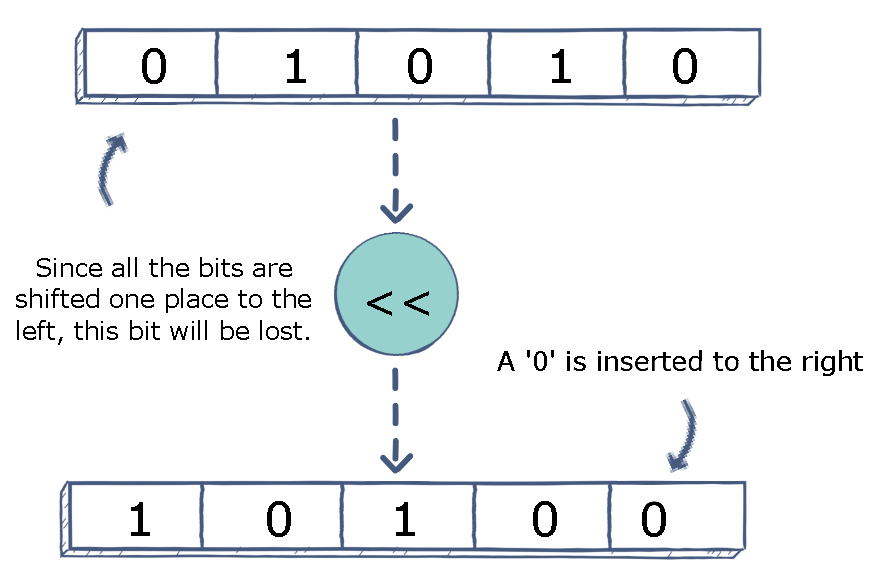
\includegraphics[width=4.25in]{leftshift.eps}
\end{center}

\subsection{Putting a Large Value in a Register}

\index{address}
\index{load}
\index{logical!shift}
\index{logical!or}
\index{move}
Often, it will be desirable to put a number larger than we can have in a single immediate into a register.  The immediate move instruction available to us only can place an $8$ bit value in a register, but registers are $32$ bits wide.

There are many ways to accomplish this, including using load instructions.  However, it can be complicated to calculate addresses.  Below is a simple method to place the value $12345678_{16}$ into \reg{0}, while using \reg{1} as a temporary space.
\vspace{0.3cm}

\renewcommand{\arraystretch}{1.5}
\begin{tabular}{p{0.1\textwidth} p{0.2\textwidth} p{0.6\textwidth}}

\texttt{20\underline{12}} & \texttt{MOV \reg{0}, $12_{16}$}&
Places the value $12_{16}$ into \reg{0}.\\

\texttt{0200} & \texttt{LSL \reg{0}, \reg{0}, \#8 }&
Shifts \reg{0} left 8 bits; it now contains $1200_{16}$.\\

\texttt{21\underline{34}} & \texttt{MOV \reg{1}, $34_{16}$}&
Puts $34_{16}$ into \reg{1}.\\

\texttt{4309} & \texttt{ORR \reg{0}, \reg{1}}&
Ors \reg{0} and \reg{1}, putting the result in \reg{0}, which now contains $1234_{16}$.\\

\texttt{0200} & \texttt{LSL \reg{0}, \reg{0}, \#8 }&
Shifts \reg{0} left 8 bits; it now contains $123400_{16}$.\\

\texttt{21\underline{56}} & \texttt{MOV \reg{1}, $56_{16}$}&
Puts $56_{16}$ into \reg{1}.\\

\texttt{4309} & \texttt{ORR \reg{0}, \reg{1}}&
Ors \reg{0} and \reg{1}, putting the result in \reg{0}, which now contains $123456_{16}$.\\

\texttt{0200} & \texttt{LSL \reg{0}, \reg{0}, \#8}&
Shifts register 0 left 8 bits; it now contains $12345600_{16}$.\\

\texttt{21\underline{78}} & \texttt{MOV \reg{1}, $78_{16}$}&
Puts $78_{16}$ into \reg{1}.\\

\texttt{4309} & \texttt{ORR \reg{0}, \reg{1}}&
Ors \reg{0} and \reg{1}, putting the result in \reg{0}, which now contains $12345678_{16}$!\\
\end{tabular}
\renewcommand{\arraystretch}{1}


\vspace{0.5cm}
In this way, we can put large numbers into any of our registers.  This approach isn't terribly efficient: 10 instructions and 20 bytes are used to load a 4 byte word into a register, but it is simple and it works.




\newpage
\section{Special (SuperVisor Call) Instructions}

\index{supervisor call}
These are special instructions that I have set up to be available on the computing environment you will use.  They provide input and output (I/O) functionality and other convenient features.

Many of these expect for an appropriate value to be loaded to $r0$ (or other registers) before executing them.

\instruction{SVC00 (toggle LED)}{If the LED is off, this turns it on.  Otherwise, it turns the LED off.}{1101 1111 0000 0000}{}{LED}

\begin{tabular}{p{0.33\textwidth} p{0.09\textwidth} p{0.44\textwidth}}
\texttt{1101 1111 0000 0000}&DF00&Basic instruction encoding\\
\end{tabular}

\instruction{SVC01 (turn LED off)}{Turns the LED off.}{1101 1111 0000 0001}{}{LED}

\begin{tabular}{p{0.33\textwidth} p{0.09\textwidth} p{0.44\textwidth}}
\texttt{1101 1111 0000 0001}&DF01&Basic instruction encoding\\
\end{tabular}

\instruction{SVC02 (turn LED on)}{Turns the LED on.}{1101 1111 0000 0010}{}{LED}

\begin{tabular}{p{0.33\textwidth} p{0.09\textwidth} p{0.44\textwidth}}
\texttt{1101 1111 0000 0010}&DF02&Basic instruction encoding\\
\end{tabular}

\instruction{SVC03 (blink the LED)}{This slowly blinks the LED.  The value in $r0$ determines how many times the LED blinks.}{1101 1111 0000 0011}{}{LED}

\begin{tabular}{p{0.33\textwidth} p{0.09\textwidth} p{0.44\textwidth}}
\texttt{1101 1111 0000 0011}&DF03&Basic instruction encoding\\
\end{tabular}

\instruction{SVC11 (sleep, tenths)}{This freezes the program for a short amount of time.  The length of time, in tenths of a second, is specified in $r0$.  For instance, if $r0$ is $15$, this will wait $1.5$ seconds before the program resumes running.}{1101 1111 0001 0001}{}{delay}

\begin{tabular}{p{0.33\textwidth} p{0.09\textwidth} p{0.44\textwidth}}
\texttt{1101 1111 0001 0001}&DF11&Basic instruction encoding\\
\end{tabular}
\newpage

\instruction{SVC12 (sleep, seconds)}{This freezes the program for a short amount of time.  The length of time, in seconds, is specified in $r0$.  For instance, if $r0$ is $15$, this will wait $15$ seconds before the program resumes running.}{1101 1111 0001 0010}{}{delay}

\begin{tabular}{p{0.33\textwidth} p{0.09\textwidth} p{0.44\textwidth}}
\texttt{1101 1111 0001 0010}&DF12&Basic instruction encoding\\
\end{tabular}

\instruction{SVC20 (clear screen)}{This clears the top half of screen and positions the cursor to write out text at the upper left.}{1101 1111 0010 0000}{}{screen}

\begin{tabular}{p{0.33\textwidth} p{0.09\textwidth} p{0.44\textwidth}}
\texttt{1101 1111 0010 0010}&DF20&Basic instruction encoding\\
\end{tabular}

\instruction{SVC21 (output number, denary)}{This prints the number in $r0$ on the screen, as a base 10 (denary) number.  For instance, if $r0$ is $F_{16}$ (or $15_{10}$), this will write the number $15$ on the screen.}{1101 1111 0010 0001}{}{screen}

\begin{tabular}{p{0.33\textwidth} p{0.09\textwidth} p{0.44\textwidth}}
\texttt{1101 1111 0010 0001}&DF21&Basic instruction encoding\\
\end{tabular}

\instruction{SVC22 (output number, hex)}{This prints the number in $r0$ on the screen, as a base 16 (hexadecimal) number.  For instance, if $r0$ is $F_{16}$ (or $15_{10}$), this will write $F$ on the screen.}{1101 1111 0010 0010}{}{screen}

\begin{tabular}{p{0.33\textwidth} p{0.09\textwidth} p{0.44\textwidth}}
\texttt{1101 1111 0010 0010}&DF22&Basic instruction encoding\\
\end{tabular}

\instruction{SVC23 (output ASCII character)}{This prints the character in $r0$ on the screen.  Only the last 8 bits of $r0$ are used.  For instance, if $r0$ is $4D_{16}$ (or $77_{10}$), this will write the character 'M' on the screen.  See the ASCII chart later in this guide for reference.}{1101 1111 0010 0011}{}{screen}

\index{ASCII}
\begin{tabular}{p{0.33\textwidth} p{0.09\textwidth} p{0.44\textwidth}}
\texttt{1101 1111 0010 0011}&DF23&Basic instruction encoding\\
\end{tabular}

\newpage
\instruction{SVC24 (draw dot)}{This changes the color of one pixel on the screen.  The color to put in the pixel is stored as an 8 bit value in $r0$.  The coordinates to change are ($r1$, $r2$).}{1101 1111 0010 0100}{}{screen}

\begin{tabular}{p{0.33\textwidth} p{0.09\textwidth} p{0.44\textwidth}}
\texttt{1101 1111 0010 0100}&DF24&Basic instruction encoding\\
\end{tabular}

\index{screen}
\instruction{SVC25 (draw icon)}{This draws a 32 byte (16 halfword) icon  on the screen.  The icon is expected to immediately follow this instruction, and when the draw is complete the instruction pointer will be increased by $22_{16}$ to skip the icon data.  The color to draw the icon is stored as an 8 bit value in $r0$. The coordinates to draw the icon at are ($r1$, $r2$).}{1101 1111 0010 0101}{}{screen}

\index{icon}

\begin{tabular}{p{0.33\textwidth} p{0.09\textwidth} p{0.44\textwidth}}
\texttt{1101 1111 0010 0101}&DF25&Basic instruction encoding (32 bytes of icon data follow)\\
\end{tabular}

\index{colors}
\subsection{Screen Colors (8-bit)}

\textbf{SVC25} and \textbf{SVC24} take in \reg{0} an 8-bit color value.  This is formatted as \texttt{RRGG GBBB},where \texttt{RR} is a two-bit value indicating the intensity of the color red, \texttt{GGG} is a three-bit value indicating the intensity of green, and \texttt{BBB} is a three-bit value indicating the intensity of the color blue.

For instance, if it's desired to draw an icon with the color purple, that requires bright red and bright blue, with no green.  Therefore, we will use the color \texttt{1100 0111} for full intensity red, no green, and full intensity blue.  This becomes the value $C7_{16}$ which can be placed into R0 with the instruction \texttt{MOV R0, F8} encoded as \texttt{20C7}.

\subsection{Screen Coordinates}

Screen drawing routines also take in coordinates in (\reg{1}, \reg{2}).  Unlike graphing coordinates, as $y$ gets bigger this moves down the screen.  The upper left corner of the screen is at ($0$, $0$).  The upper right of the screen is at ($160$, $0$).  The bottommost row you should draw on is row $53$, which means the other two corners are at ($0$, $53$) and ($160$, $53$).

\section{Miscellaneous Reference}
\subsection{ASCII Character Map}
\index{ASCII}
\begin{center}
%%%%%%%%%%%%%%%%%%%%%%%%%%%%%%%%%%%%%%%%%%%%%%%%%%%%%%%%%%%%%%%%%%%%%%%%
%%                                                                    %%
%%                     A S C I I    wall chart                        %%
%%                                                                    %%
%% by Victor Eijkhout                                                 %%
%% victor@eijkhout.net                                                %%
%%                                                                    %%
%%%%%%%%%%%%%%%%%%%%%%%%%%%%%%%%%%%%%%%%%%%%%%%%%%%%%%%%%%%%%%%%%%%%%%%%
%% Copyright 2009 Victor Eijkhout
%
% This work may be distributed and/or modified under the
% conditions of the LaTeX Project Public License, either version 1.3
% of this license or (at your option) any later version.
% The latest version of this license is in
%   http://www.latex-project.org/lppl.txt
% and version 1.3 or later is part of all distributions of LaTeX
% version 2005/12/01 or later.
%
% This work has the LPPL maintenance status `maintained'.
% 
% The Current Maintainer of this work is Victor Eijkhout.
%
% This work consists of this file.
%
%% Choose your favourite format:
%
%\nopagenumbers %% 2 lines
%\vsize=28cm    %% for PLAIN TeX
%\documentstyle{article}            %% 4 lines for LaTeX
%\begin{document}                   %% not that it matters anything,
%\pagestyle{empty}                  %% rest of the document
%\setlength{\textheight}{28cm}      %% is 'pure' TeX.
%%%%%% and don't forget the \bye / \end{document} at the end!! %%%%%%%
%% fonts
\font\bitfont=cmr10 \fontdimen4\bitfont=3mm
\font\codefont=cmr7
\font\namefont=cmss10 scaled 1200
\font\titlefont=cmss10 scaled 1440
\font\commentfont=cmss10
%% counts and dimens
\newdimen\thinlinewidth \thinlinewidth=.25mm
\newdimen\fatlinewidth \fatlinewidth=.5mm
\newdimen\rowheight \rowheight=0.95cm
\newdimen\colwidth  \colwidth=1.6cm
\newdimen\Colwidth \Colwidth=2\colwidth
  \advance\Colwidth by \thinlinewidth
\newdimen\topwhite \topwhite=2pt
\newdimen\botwhite \botwhite=3pt
\newdimen\leftwhite \leftwhite=2pt
\newdimen\rightwhite \rightwhite=2pt
\newcount\rowcount \rowcount=-1 %% note!
\newcount\colcount \colcount=0
\newcount\thenumber
%% tidbits
\def\\{$\backslash$}
\def\thinline{\vrule width \thinlinewidth}
\def\fatline{\vrule width \fatlinewidth}
\tolerance=10000
\vbadness=10000
%% code conversion
\def\calcnumber{{\multiply\colcount by 16
                 \advance\colcount by \rowcount
                 \global\thenumber=\colcount}}
\def\deccode{\number\thenumber}
\def\octcode{{\ifnum\thenumber>63
                            \advance\thenumber by -64
                            \count0=\thenumber \divide\count0 by 8
                            1\number\count0
              \else         \count0=\thenumber \divide\count0 by 8
                            \ifnum\count0>0 \number\count0 \fi\fi
              \multiply\count0 by 8
              \advance\thenumber by -\count0
              \number\thenumber}}
\def\hexdigit#1{\ifcase#1 0\or 1\or 2\or 3\or 4\or 5\or 6\or 7\or
                          8\or 9\or A\or B\or C\or D\or E\or F\or
                          \edef\tmp{\message{illegal hex digit
                                        \number#1}}\tmp
                          \fi}
\def\hexcode{{\count0=\thenumber \divide\count0 by 16
              \ifnum\count0>0 \hexdigit{\count0}\fi
              \multiply\count0 by 16
              \advance\thenumber by -\count0 \count0=\thenumber
              \hexdigit{\count0}}}
%% the heading
\def\threebit#1#2#3{\vbox to 1.5\rowheight{\bitfont
                      \vskip\topwhite
                      \hbox to \colwidth{\hskip\leftwhite#1\hfil}
                      \vfil
                      \hbox to \colwidth{\hfil#2\hfil}
                      \vfil
                      \hbox to \colwidth{\hfil#3\hskip\rightwhite}
                      \vskip\botwhite}}
\def\comment#1{\vbox to \colwidth{\hrule height 0mm depth .25mm
                      \vfil
                      \hbox to \Colwidth{\commentfont\hfil#1\hfil}
                      \vfil}}
\def\dcomment#1#2{\vbox to \colwidth{\hrule height 0mm depth .25mm
                      \vfil
                      \hbox to \Colwidth{\commentfont\hfil#1\hfil}
                      \vskip \botwhite
                      \hbox to \Colwidth{\commentfont\hfil#2\hfil}
                      \vfil}}
\def\bithead{\vbox to \colwidth{\hsize=1.5\colwidth
                   \vskip\topwhite
                   \hbox to \hsize{\commentfont\hfil BITS\hfil}
                   \vfil
                   \hbox to \hsize{\bitfont\ b4 b3 b2 b1 }
                   \vskip\botwhite}}
%% routines for single chars
\def\fourbit#1\fb{\vbox to \rowheight{
                     \vfil
                     \hbox to 1.5\colwidth{\bitfont #1\ }
                     \vfil}%
                  \global\advance\rowcount by 1
                  \global\colcount=0}
\def\asc#1\ii{\calcnumber
              \vbox to \rowheight{\offinterlineskip
                     \vskip\topwhite
                     \hbox to \colwidth{\codefont
                                        \hskip\leftwhite
                                        \deccode\hfil}
                     \vfil
                     \hbox to \colwidth{\vrule width 0cm
                                              height 10pt depth 2pt
                                        \namefont
                                        \hfil#1\hfil}
                     \vfil
                     \hbox to \colwidth{\codefont
                                        \hskip\leftwhite
                                        \hexcode\hfil %\octcode
                                        \hskip\rightwhite}
                     \vskip\botwhite}%
              \global\advance\colcount by 1}
%%%%%%%%%%%%%%%%% and now the table itself %%%%%%%%%%%%%%%%%%%%%%%%%
\vbox{
\halign{\fatline\fourbit#\fb&\fatline\asc#\ii&\thinline\asc#\ii&
                     \fatline\asc#\ii&\thinline\asc#\ii&
                     \fatline\asc#\ii&\thinline\asc#\ii&
                     \fatline\asc#\ii&\thinline\asc#\ii\fatline\cr
          \omit&\multispan8 \hskip\thinlinewidth
                            \titlefont
                            %ASCII CONTROL CODE CHART
                            \hfil\cr
    \noalign{\vskip4mm\hrule}
          \omit\fatline\hfil\threebit{b7}{b6}{b5}
                 &\omit\fatline\threebit000&\omit\thinline\threebit001%
                 &\omit\fatline\threebit010&\omit\thinline\threebit011%
                 &\omit\fatline\threebit100&\omit\thinline\threebit101%
                 &\omit\fatline\threebit110&\omit\thinline\threebit111%
                                                 \fatline\cr
    \noalign{\vskip-.5mm} %brute force
          \omit\fatline\bithead
                 &\omit\fatline\comment{CONTROL}\span\omit
                 &\omit\fatline\dcomment{SYMBOLS}{NUMBERS}\span\omit
                 &\omit\fatline\comment{UPPER CASE}\span\omit
                 &\omit\fatline\comment{LOWER CASE}\span\omit\hfil\fatline\cr
    \noalign{\hrule}
      {} 0 0 0 0&NUL&DLE&SP     &0  &@  &P       &` &p  \cr\noalign{\hrule}
      {} 0 0 0 1&SOH&DC1&!      &1  &A  &Q       &a &q  \cr\noalign{\hrule}
      {} 0 0 1 0&STX&DC2&"      &2  &B  &R       &b &r  \cr\noalign{\hrule}
      {} 0 0 1 1&ETX&DC3&\#     &3  &C  &S       &c &s  \cr\noalign{\hrule}
      {} 0 1 0 0&EOT&DC4&\$     &4  &D  &T       &d &t  \cr\noalign{\hrule}
      {} 0 1 0 1&ENQ&NAK&\%     &5  &E  &U       &e &u  \cr\noalign{\hrule}
      {} 0 1 1 0&ACK&SYN&\&     &6  &F  &V       &f &v  \cr\noalign{\hrule}
      {} 0 1 1 1&BEL&ETB&'      &7  &G  &W       &g &w  \cr\noalign{\hrule}
      {} 1 0 0 0&BS &CAN&(      &8  &H  &X       &h &x  \cr\noalign{\hrule}
      {} 1 0 0 1&HT &EM &)      &9  &I  &Y       &i &y  \cr\noalign{\hrule}
      {} 1 0 1 0&LF &SUB&*      &:  &J  &Z       &j &z  \cr\noalign{\hrule}
      {} 1 0 1 1&VT &ESC&+      &;  &K  &[       &k &$\{$\cr  \noalign{\hrule}
      {} 1 1 0 0&FF &FS &,      &$<$&L  &\\      &l &$|$ \cr  \noalign{\hrule}
      {} 1 1 0 1&CR &GS &$-$    &=  &M  &]       &m &$\}$\cr  \noalign{\hrule}
      {} 1 1 1 0&SO &RS &.      &$>$&N  &\char94 &n &\char126\cr
                    \noalign{\hrule}
      {} 1 1 1 1&SI &US &/      &?  &O  &\_$\!$\_&o &DEL\cr\noalign{\hrule}
   \noalign{\vskip2mm}
          \omit&\omit\namefont \hfil LEGEND:\hfil \span\omit
          &\multispan4\hskip\fatlinewidth
            \vtop{\vskip-10pt\hbox{\vrule
             \vbox to \rowheight{
                 \offinterlineskip
                 \hrule\vskip \topwhite
                 \hbox to \colwidth{\codefont\hskip\leftwhite
                                       dec\hfil}
                 \vfil
                 \hbox to \colwidth{\namefont\hfil CHAR\hfil}
                 \vfil
                 \hbox to \colwidth{\codefont\hskip\leftwhite
                                       hex\hfil
                                       \hskip\rightwhite}
                 \vskip\botwhite
                 \hrule                               }%
                                  \vrule}}
                      \hfil
          &\multispan2\bitfont \hskip\fatlinewidth
                      \vtop{\vskip-8pt\baselineskip=8.5pt
                            \hbox{Victor Eijkhout}
                            \rlap{Dept. of Comp. Sci.}
                            \rlap{University of Tennessee}
                            \rlap{Knoxville TN 37996, USA}
                            }\hfil\cr
          }
}
%%%%%%%%%%%%%%%%%%%%%%% and that's it folks! %%%%%%%%%%%%%%%%%%%%%%%%%%

%\bye          %% PLAIN TeX
%\end{document} %% LaTeX

(modified by Michael Lyle, 2021)
\end{center}

\newpage
\subsection{ARM Thumb Instruction Encoding}
\index{instruction encodings}
\vspace{0.5cm}
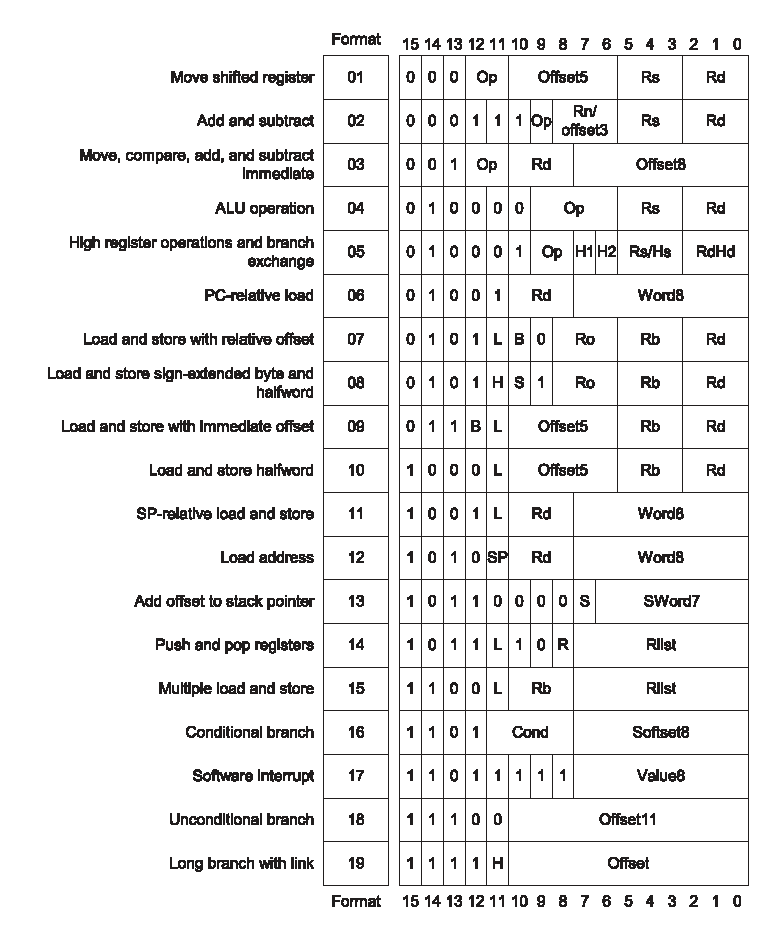
\includegraphics[width=\textwidth]{insencoding.eps}
Source: DDI0210, Arm Limited, 2004

\newpage
\subsection{Hexadecimal and Decimal Conversion (Nybbles)}
\index{nybble}
\begin{tabular}{p{0.16\textwidth} p{0.16\textwidth} p{0.16\textwidth}}
\index{decimal}Decimal & \index{binary}Binary & \index{hexadecimal}Hexadecimal\\
\hline
$0$ & \numtt{0000} & $0$\\
$1$ & \numtt{0001} & $1$\\
$2$ & \numtt{0010} & $2$\\
$3$ & \numtt{0011} & $3$\\
$4$ & \numtt{0100} & $4$\\
$5$ & \numtt{0101} & $5$\\
$6$ & \numtt{0110} & $6$\\
$7$ & \numtt{0111} & $7$\\
$8$ & \numtt{1000} & $8$\\
$9$ & \numtt{1001} & $9$\\
$10$ & \numtt{1010} & $A$\\
$11$ & \numtt{1011} & $B$\\
$12$ & \numtt{1100} & $C$\\
$13$ & \numtt{1101} & $D$\\
$14$ & \numtt{1110} & $E$\\
$15$ & \numtt{1111} & $F$\\
\end{tabular}

\index{branch!offsets}
\subsection{Branch Offsets (as used in B, BNZ, etc.)}
\begin{tabular}{p{0.25\textwidth} p{0.12\textwidth} p{0.23\textwidth} p{0.23\textwidth}}
Number of Instructions & Address Offset & 8 Bit Conditional Branch Offset & 11 Bit Branch Offset\\
\hline
Back 30 & $-3C_{16}$ & $E0_{16}$ & $7E0_{16}$ \\
Back 29 & $-3A_{16}$ & $E1_{16}$ & $7E1_{16}$ \\
...\\
Back 16 & $-20_{16}$ & $EE_{16}$ & $7EE_{16}$ \\
Back 15 & $-1E_{16}$ & $EF_{16}$ & $7EF_{16}$ \\
Back 14 & $-1C_{16}$ & $F0_{16}$ & $7F0_{16}$ \\
Back 13 & $-1A_{16}$ & $F1_{16}$ & $7F1_{16}$ \\
Back 12 & $-18_{16}$ & $F2_{16}$ & $7F2_{16}$ \\
...\\
Back 2 & $-4_{16}$ & $FC_{16}$ & $7FC_{16}$ \\
Back 1 & $-2_{16}$ & $FD_{16}$ & $7FD_{16}$ \\
Infinite Loop & $0$ & $FE_{16}$ & $7FE_{16}$ \\
Forward 1 (Do Nothing) & $+2_{16}$ & $FF_{16}$ & $7FF_{16}$ \\
Forward 2 (Skip 1) & $+4_{16}$ & $00_{16}$ & $000_{16}$ \\
Forward 3 (Skip 2) & $+6_{16}$ & $01_{16}$ & $001_{16}$ \\
...\\
Forward 15 (Skip 14) & $+1E_{16}$ & $0E_{16}$ & $00E_{16}$ \\
Forward 16 (Skip 15) & $+20_{16}$ & $0F_{16}$ & $00F_{16}$ \\
Forward 17 (Skip 16) & $+22_{16}$ & $10_{16}$ & $010_{16}$ \\
Forward 18 (Skip 17) & $+24_{16}$ & $11_{16}$ & $011_{16}$
\end{tabular}


\newpage
\addcontentsline{toc}{subsection}{ARM Thumb-16 Quick Reference Card}
\index{add}
\index{move}
\index{subtract}
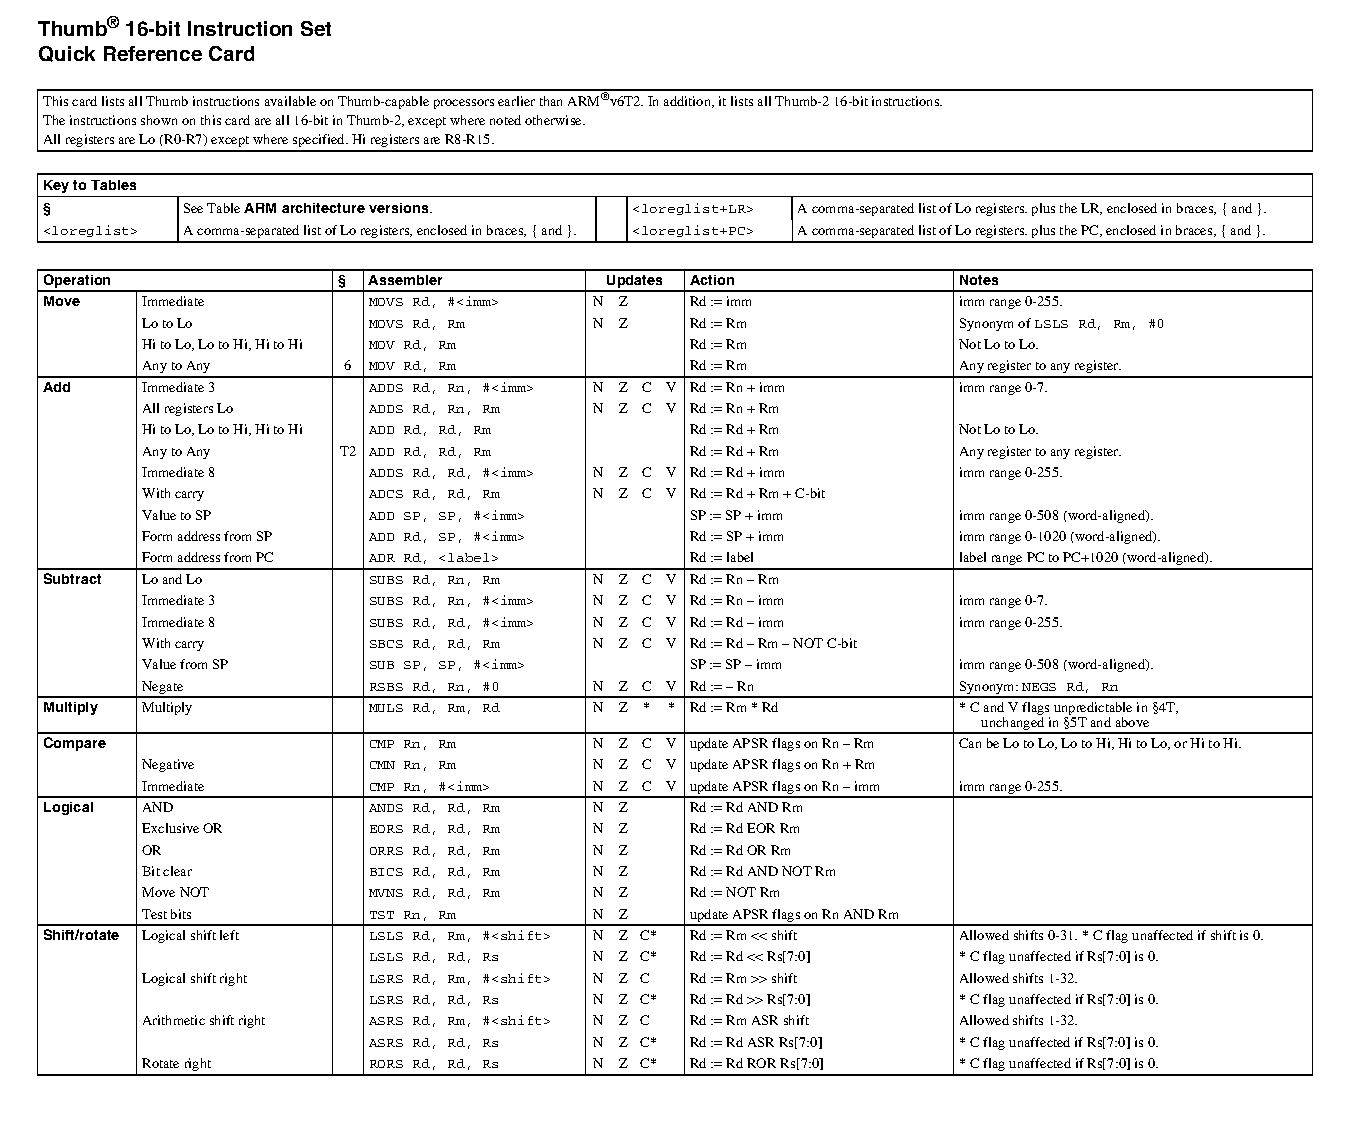
\includepdf[angle=90,pages=1,pagecommand={},width=7.65in, offset=0.25in 0]{ThumbRefCard.pdf}
\index{load}
\index{address}
\index{store}
\index{branch}
\index{logical!and}
\index{logical!or}
\index{logical!shift}
\includepdf[angle=90,pages=2,pagecommand={},width=7.65in, offset=0.25in 0]{ThumbRefCard.pdf}
\index{supervisor call}
\includepdf[angle=90,pages=3,pagecommand={},width=7.65in, offset=0.25in 0]{ThumbRefCard.pdf}


\printindex

\end{document}
